\documentclass[11pt]{article}

    \usepackage[breakable]{tcolorbox}
    \usepackage{parskip} % Stop auto-indenting (to mimic markdown behaviour)
    
    \usepackage{iftex}
    \ifPDFTeX
    	\usepackage[T1]{fontenc}
    	\usepackage{mathpazo}
    \else
    	\usepackage{fontspec}
    \fi

    % Basic figure setup, for now with no caption control since it's done
    % automatically by Pandoc (which extracts ![](path) syntax from Markdown).
    \usepackage{graphicx}
    % Maintain compatibility with old templates. Remove in nbconvert 6.0
    \let\Oldincludegraphics\includegraphics
    % Ensure that by default, figures have no caption (until we provide a
    % proper Figure object with a Caption API and a way to capture that
    % in the conversion process - todo).
    \usepackage{caption}
    \DeclareCaptionFormat{nocaption}{}
    \captionsetup{format=nocaption,aboveskip=0pt,belowskip=0pt}

    \usepackage{float}
    \floatplacement{figure}{H} % forces figures to be placed at the correct location
    \usepackage{xcolor} % Allow colors to be defined
    \usepackage{enumerate} % Needed for markdown enumerations to work
    \usepackage{geometry} % Used to adjust the document margins
    \usepackage{amsmath} % Equations
    \usepackage{amssymb} % Equations
    \usepackage{textcomp} % defines textquotesingle
    % Hack from http://tex.stackexchange.com/a/47451/13684:
    \AtBeginDocument{%
        \def\PYZsq{\textquotesingle}% Upright quotes in Pygmentized code
    }
    \usepackage{upquote} % Upright quotes for verbatim code
    \usepackage{eurosym} % defines \euro
    \usepackage[mathletters]{ucs} % Extended unicode (utf-8) support
    \usepackage{fancyvrb} % verbatim replacement that allows latex
    \usepackage{grffile} % extends the file name processing of package graphics 
                         % to support a larger range
    \makeatletter % fix for old versions of grffile with XeLaTeX
    \@ifpackagelater{grffile}{2019/11/01}
    {
      % Do nothing on new versions
    }
    {
      \def\Gread@@xetex#1{%
        \IfFileExists{"\Gin@base".bb}%
        {\Gread@eps{\Gin@base.bb}}%
        {\Gread@@xetex@aux#1}%
      }
    }
    \makeatother
    \usepackage[Export]{adjustbox} % Used to constrain images to a maximum size
    \adjustboxset{max size={0.9\linewidth}{0.9\paperheight}}

    % The hyperref package gives us a pdf with properly built
    % internal navigation ('pdf bookmarks' for the table of contents,
    % internal cross-reference links, web links for URLs, etc.)
    \usepackage{hyperref}
    % The default LaTeX title has an obnoxious amount of whitespace. By default,
    % titling removes some of it. It also provides customization options.
    \usepackage{titling}
    \usepackage{longtable} % longtable support required by pandoc >1.10
    \usepackage{booktabs}  % table support for pandoc > 1.12.2
    \usepackage[inline]{enumitem} % IRkernel/repr support (it uses the enumerate* environment)
    \usepackage[normalem]{ulem} % ulem is needed to support strikethroughs (\sout)
                                % normalem makes italics be italics, not underlines
    \usepackage{mathrsfs}
    

    
    % Colors for the hyperref package
    \definecolor{urlcolor}{rgb}{0,.145,.698}
    \definecolor{linkcolor}{rgb}{.71,0.21,0.01}
    \definecolor{citecolor}{rgb}{.12,.54,.11}

    % ANSI colors
    \definecolor{ansi-black}{HTML}{3E424D}
    \definecolor{ansi-black-intense}{HTML}{282C36}
    \definecolor{ansi-red}{HTML}{E75C58}
    \definecolor{ansi-red-intense}{HTML}{B22B31}
    \definecolor{ansi-green}{HTML}{00A250}
    \definecolor{ansi-green-intense}{HTML}{007427}
    \definecolor{ansi-yellow}{HTML}{DDB62B}
    \definecolor{ansi-yellow-intense}{HTML}{B27D12}
    \definecolor{ansi-blue}{HTML}{208FFB}
    \definecolor{ansi-blue-intense}{HTML}{0065CA}
    \definecolor{ansi-magenta}{HTML}{D160C4}
    \definecolor{ansi-magenta-intense}{HTML}{A03196}
    \definecolor{ansi-cyan}{HTML}{60C6C8}
    \definecolor{ansi-cyan-intense}{HTML}{258F8F}
    \definecolor{ansi-white}{HTML}{C5C1B4}
    \definecolor{ansi-white-intense}{HTML}{A1A6B2}
    \definecolor{ansi-default-inverse-fg}{HTML}{FFFFFF}
    \definecolor{ansi-default-inverse-bg}{HTML}{000000}

    % common color for the border for error outputs.
    \definecolor{outerrorbackground}{HTML}{FFDFDF}

    % commands and environments needed by pandoc snippets
    % extracted from the output of `pandoc -s`
    \providecommand{\tightlist}{%
      \setlength{\itemsep}{0pt}\setlength{\parskip}{0pt}}
    \DefineVerbatimEnvironment{Highlighting}{Verbatim}{commandchars=\\\{\}}
    % Add ',fontsize=\small' for more characters per line
    \newenvironment{Shaded}{}{}
    \newcommand{\KeywordTok}[1]{\textcolor[rgb]{0.00,0.44,0.13}{\textbf{{#1}}}}
    \newcommand{\DataTypeTok}[1]{\textcolor[rgb]{0.56,0.13,0.00}{{#1}}}
    \newcommand{\DecValTok}[1]{\textcolor[rgb]{0.25,0.63,0.44}{{#1}}}
    \newcommand{\BaseNTok}[1]{\textcolor[rgb]{0.25,0.63,0.44}{{#1}}}
    \newcommand{\FloatTok}[1]{\textcolor[rgb]{0.25,0.63,0.44}{{#1}}}
    \newcommand{\CharTok}[1]{\textcolor[rgb]{0.25,0.44,0.63}{{#1}}}
    \newcommand{\StringTok}[1]{\textcolor[rgb]{0.25,0.44,0.63}{{#1}}}
    \newcommand{\CommentTok}[1]{\textcolor[rgb]{0.38,0.63,0.69}{\textit{{#1}}}}
    \newcommand{\OtherTok}[1]{\textcolor[rgb]{0.00,0.44,0.13}{{#1}}}
    \newcommand{\AlertTok}[1]{\textcolor[rgb]{1.00,0.00,0.00}{\textbf{{#1}}}}
    \newcommand{\FunctionTok}[1]{\textcolor[rgb]{0.02,0.16,0.49}{{#1}}}
    \newcommand{\RegionMarkerTok}[1]{{#1}}
    \newcommand{\ErrorTok}[1]{\textcolor[rgb]{1.00,0.00,0.00}{\textbf{{#1}}}}
    \newcommand{\NormalTok}[1]{{#1}}
    
    % Additional commands for more recent versions of Pandoc
    \newcommand{\ConstantTok}[1]{\textcolor[rgb]{0.53,0.00,0.00}{{#1}}}
    \newcommand{\SpecialCharTok}[1]{\textcolor[rgb]{0.25,0.44,0.63}{{#1}}}
    \newcommand{\VerbatimStringTok}[1]{\textcolor[rgb]{0.25,0.44,0.63}{{#1}}}
    \newcommand{\SpecialStringTok}[1]{\textcolor[rgb]{0.73,0.40,0.53}{{#1}}}
    \newcommand{\ImportTok}[1]{{#1}}
    \newcommand{\DocumentationTok}[1]{\textcolor[rgb]{0.73,0.13,0.13}{\textit{{#1}}}}
    \newcommand{\AnnotationTok}[1]{\textcolor[rgb]{0.38,0.63,0.69}{\textbf{\textit{{#1}}}}}
    \newcommand{\CommentVarTok}[1]{\textcolor[rgb]{0.38,0.63,0.69}{\textbf{\textit{{#1}}}}}
    \newcommand{\VariableTok}[1]{\textcolor[rgb]{0.10,0.09,0.49}{{#1}}}
    \newcommand{\ControlFlowTok}[1]{\textcolor[rgb]{0.00,0.44,0.13}{\textbf{{#1}}}}
    \newcommand{\OperatorTok}[1]{\textcolor[rgb]{0.40,0.40,0.40}{{#1}}}
    \newcommand{\BuiltInTok}[1]{{#1}}
    \newcommand{\ExtensionTok}[1]{{#1}}
    \newcommand{\PreprocessorTok}[1]{\textcolor[rgb]{0.74,0.48,0.00}{{#1}}}
    \newcommand{\AttributeTok}[1]{\textcolor[rgb]{0.49,0.56,0.16}{{#1}}}
    \newcommand{\InformationTok}[1]{\textcolor[rgb]{0.38,0.63,0.69}{\textbf{\textit{{#1}}}}}
    \newcommand{\WarningTok}[1]{\textcolor[rgb]{0.38,0.63,0.69}{\textbf{\textit{{#1}}}}}
    
    
    % Define a nice break command that doesn't care if a line doesn't already
    % exist.
    \def\br{\hspace*{\fill} \\* }
    % Math Jax compatibility definitions
    \def\gt{>}
    \def\lt{<}
    \let\Oldtex\TeX
    \let\Oldlatex\LaTeX
    \renewcommand{\TeX}{\textrm{\Oldtex}}
    \renewcommand{\LaTeX}{\textrm{\Oldlatex}}
    % Document parameters
    % Document title
    \title{8.2 Motion Planning with Potential Fields}
    
    
    
    
    
% Pygments definitions
\makeatletter
\def\PY@reset{\let\PY@it=\relax \let\PY@bf=\relax%
    \let\PY@ul=\relax \let\PY@tc=\relax%
    \let\PY@bc=\relax \let\PY@ff=\relax}
\def\PY@tok#1{\csname PY@tok@#1\endcsname}
\def\PY@toks#1+{\ifx\relax#1\empty\else%
    \PY@tok{#1}\expandafter\PY@toks\fi}
\def\PY@do#1{\PY@bc{\PY@tc{\PY@ul{%
    \PY@it{\PY@bf{\PY@ff{#1}}}}}}}
\def\PY#1#2{\PY@reset\PY@toks#1+\relax+\PY@do{#2}}

\expandafter\def\csname PY@tok@w\endcsname{\def\PY@tc##1{\textcolor[rgb]{0.73,0.73,0.73}{##1}}}
\expandafter\def\csname PY@tok@c\endcsname{\let\PY@it=\textit\def\PY@tc##1{\textcolor[rgb]{0.25,0.50,0.50}{##1}}}
\expandafter\def\csname PY@tok@cp\endcsname{\def\PY@tc##1{\textcolor[rgb]{0.74,0.48,0.00}{##1}}}
\expandafter\def\csname PY@tok@k\endcsname{\let\PY@bf=\textbf\def\PY@tc##1{\textcolor[rgb]{0.00,0.50,0.00}{##1}}}
\expandafter\def\csname PY@tok@kp\endcsname{\def\PY@tc##1{\textcolor[rgb]{0.00,0.50,0.00}{##1}}}
\expandafter\def\csname PY@tok@kt\endcsname{\def\PY@tc##1{\textcolor[rgb]{0.69,0.00,0.25}{##1}}}
\expandafter\def\csname PY@tok@o\endcsname{\def\PY@tc##1{\textcolor[rgb]{0.40,0.40,0.40}{##1}}}
\expandafter\def\csname PY@tok@ow\endcsname{\let\PY@bf=\textbf\def\PY@tc##1{\textcolor[rgb]{0.67,0.13,1.00}{##1}}}
\expandafter\def\csname PY@tok@nb\endcsname{\def\PY@tc##1{\textcolor[rgb]{0.00,0.50,0.00}{##1}}}
\expandafter\def\csname PY@tok@nf\endcsname{\def\PY@tc##1{\textcolor[rgb]{0.00,0.00,1.00}{##1}}}
\expandafter\def\csname PY@tok@nc\endcsname{\let\PY@bf=\textbf\def\PY@tc##1{\textcolor[rgb]{0.00,0.00,1.00}{##1}}}
\expandafter\def\csname PY@tok@nn\endcsname{\let\PY@bf=\textbf\def\PY@tc##1{\textcolor[rgb]{0.00,0.00,1.00}{##1}}}
\expandafter\def\csname PY@tok@ne\endcsname{\let\PY@bf=\textbf\def\PY@tc##1{\textcolor[rgb]{0.82,0.25,0.23}{##1}}}
\expandafter\def\csname PY@tok@nv\endcsname{\def\PY@tc##1{\textcolor[rgb]{0.10,0.09,0.49}{##1}}}
\expandafter\def\csname PY@tok@no\endcsname{\def\PY@tc##1{\textcolor[rgb]{0.53,0.00,0.00}{##1}}}
\expandafter\def\csname PY@tok@nl\endcsname{\def\PY@tc##1{\textcolor[rgb]{0.63,0.63,0.00}{##1}}}
\expandafter\def\csname PY@tok@ni\endcsname{\let\PY@bf=\textbf\def\PY@tc##1{\textcolor[rgb]{0.60,0.60,0.60}{##1}}}
\expandafter\def\csname PY@tok@na\endcsname{\def\PY@tc##1{\textcolor[rgb]{0.49,0.56,0.16}{##1}}}
\expandafter\def\csname PY@tok@nt\endcsname{\let\PY@bf=\textbf\def\PY@tc##1{\textcolor[rgb]{0.00,0.50,0.00}{##1}}}
\expandafter\def\csname PY@tok@nd\endcsname{\def\PY@tc##1{\textcolor[rgb]{0.67,0.13,1.00}{##1}}}
\expandafter\def\csname PY@tok@s\endcsname{\def\PY@tc##1{\textcolor[rgb]{0.73,0.13,0.13}{##1}}}
\expandafter\def\csname PY@tok@sd\endcsname{\let\PY@it=\textit\def\PY@tc##1{\textcolor[rgb]{0.73,0.13,0.13}{##1}}}
\expandafter\def\csname PY@tok@si\endcsname{\let\PY@bf=\textbf\def\PY@tc##1{\textcolor[rgb]{0.73,0.40,0.53}{##1}}}
\expandafter\def\csname PY@tok@se\endcsname{\let\PY@bf=\textbf\def\PY@tc##1{\textcolor[rgb]{0.73,0.40,0.13}{##1}}}
\expandafter\def\csname PY@tok@sr\endcsname{\def\PY@tc##1{\textcolor[rgb]{0.73,0.40,0.53}{##1}}}
\expandafter\def\csname PY@tok@ss\endcsname{\def\PY@tc##1{\textcolor[rgb]{0.10,0.09,0.49}{##1}}}
\expandafter\def\csname PY@tok@sx\endcsname{\def\PY@tc##1{\textcolor[rgb]{0.00,0.50,0.00}{##1}}}
\expandafter\def\csname PY@tok@m\endcsname{\def\PY@tc##1{\textcolor[rgb]{0.40,0.40,0.40}{##1}}}
\expandafter\def\csname PY@tok@gh\endcsname{\let\PY@bf=\textbf\def\PY@tc##1{\textcolor[rgb]{0.00,0.00,0.50}{##1}}}
\expandafter\def\csname PY@tok@gu\endcsname{\let\PY@bf=\textbf\def\PY@tc##1{\textcolor[rgb]{0.50,0.00,0.50}{##1}}}
\expandafter\def\csname PY@tok@gd\endcsname{\def\PY@tc##1{\textcolor[rgb]{0.63,0.00,0.00}{##1}}}
\expandafter\def\csname PY@tok@gi\endcsname{\def\PY@tc##1{\textcolor[rgb]{0.00,0.63,0.00}{##1}}}
\expandafter\def\csname PY@tok@gr\endcsname{\def\PY@tc##1{\textcolor[rgb]{1.00,0.00,0.00}{##1}}}
\expandafter\def\csname PY@tok@ge\endcsname{\let\PY@it=\textit}
\expandafter\def\csname PY@tok@gs\endcsname{\let\PY@bf=\textbf}
\expandafter\def\csname PY@tok@gp\endcsname{\let\PY@bf=\textbf\def\PY@tc##1{\textcolor[rgb]{0.00,0.00,0.50}{##1}}}
\expandafter\def\csname PY@tok@go\endcsname{\def\PY@tc##1{\textcolor[rgb]{0.53,0.53,0.53}{##1}}}
\expandafter\def\csname PY@tok@gt\endcsname{\def\PY@tc##1{\textcolor[rgb]{0.00,0.27,0.87}{##1}}}
\expandafter\def\csname PY@tok@err\endcsname{\def\PY@bc##1{\setlength{\fboxsep}{0pt}\fcolorbox[rgb]{1.00,0.00,0.00}{1,1,1}{\strut ##1}}}
\expandafter\def\csname PY@tok@kc\endcsname{\let\PY@bf=\textbf\def\PY@tc##1{\textcolor[rgb]{0.00,0.50,0.00}{##1}}}
\expandafter\def\csname PY@tok@kd\endcsname{\let\PY@bf=\textbf\def\PY@tc##1{\textcolor[rgb]{0.00,0.50,0.00}{##1}}}
\expandafter\def\csname PY@tok@kn\endcsname{\let\PY@bf=\textbf\def\PY@tc##1{\textcolor[rgb]{0.00,0.50,0.00}{##1}}}
\expandafter\def\csname PY@tok@kr\endcsname{\let\PY@bf=\textbf\def\PY@tc##1{\textcolor[rgb]{0.00,0.50,0.00}{##1}}}
\expandafter\def\csname PY@tok@bp\endcsname{\def\PY@tc##1{\textcolor[rgb]{0.00,0.50,0.00}{##1}}}
\expandafter\def\csname PY@tok@fm\endcsname{\def\PY@tc##1{\textcolor[rgb]{0.00,0.00,1.00}{##1}}}
\expandafter\def\csname PY@tok@vc\endcsname{\def\PY@tc##1{\textcolor[rgb]{0.10,0.09,0.49}{##1}}}
\expandafter\def\csname PY@tok@vg\endcsname{\def\PY@tc##1{\textcolor[rgb]{0.10,0.09,0.49}{##1}}}
\expandafter\def\csname PY@tok@vi\endcsname{\def\PY@tc##1{\textcolor[rgb]{0.10,0.09,0.49}{##1}}}
\expandafter\def\csname PY@tok@vm\endcsname{\def\PY@tc##1{\textcolor[rgb]{0.10,0.09,0.49}{##1}}}
\expandafter\def\csname PY@tok@sa\endcsname{\def\PY@tc##1{\textcolor[rgb]{0.73,0.13,0.13}{##1}}}
\expandafter\def\csname PY@tok@sb\endcsname{\def\PY@tc##1{\textcolor[rgb]{0.73,0.13,0.13}{##1}}}
\expandafter\def\csname PY@tok@sc\endcsname{\def\PY@tc##1{\textcolor[rgb]{0.73,0.13,0.13}{##1}}}
\expandafter\def\csname PY@tok@dl\endcsname{\def\PY@tc##1{\textcolor[rgb]{0.73,0.13,0.13}{##1}}}
\expandafter\def\csname PY@tok@s2\endcsname{\def\PY@tc##1{\textcolor[rgb]{0.73,0.13,0.13}{##1}}}
\expandafter\def\csname PY@tok@sh\endcsname{\def\PY@tc##1{\textcolor[rgb]{0.73,0.13,0.13}{##1}}}
\expandafter\def\csname PY@tok@s1\endcsname{\def\PY@tc##1{\textcolor[rgb]{0.73,0.13,0.13}{##1}}}
\expandafter\def\csname PY@tok@mb\endcsname{\def\PY@tc##1{\textcolor[rgb]{0.40,0.40,0.40}{##1}}}
\expandafter\def\csname PY@tok@mf\endcsname{\def\PY@tc##1{\textcolor[rgb]{0.40,0.40,0.40}{##1}}}
\expandafter\def\csname PY@tok@mh\endcsname{\def\PY@tc##1{\textcolor[rgb]{0.40,0.40,0.40}{##1}}}
\expandafter\def\csname PY@tok@mi\endcsname{\def\PY@tc##1{\textcolor[rgb]{0.40,0.40,0.40}{##1}}}
\expandafter\def\csname PY@tok@il\endcsname{\def\PY@tc##1{\textcolor[rgb]{0.40,0.40,0.40}{##1}}}
\expandafter\def\csname PY@tok@mo\endcsname{\def\PY@tc##1{\textcolor[rgb]{0.40,0.40,0.40}{##1}}}
\expandafter\def\csname PY@tok@ch\endcsname{\let\PY@it=\textit\def\PY@tc##1{\textcolor[rgb]{0.25,0.50,0.50}{##1}}}
\expandafter\def\csname PY@tok@cm\endcsname{\let\PY@it=\textit\def\PY@tc##1{\textcolor[rgb]{0.25,0.50,0.50}{##1}}}
\expandafter\def\csname PY@tok@cpf\endcsname{\let\PY@it=\textit\def\PY@tc##1{\textcolor[rgb]{0.25,0.50,0.50}{##1}}}
\expandafter\def\csname PY@tok@c1\endcsname{\let\PY@it=\textit\def\PY@tc##1{\textcolor[rgb]{0.25,0.50,0.50}{##1}}}
\expandafter\def\csname PY@tok@cs\endcsname{\let\PY@it=\textit\def\PY@tc##1{\textcolor[rgb]{0.25,0.50,0.50}{##1}}}

\def\PYZbs{\char`\\}
\def\PYZus{\char`\_}
\def\PYZob{\char`\{}
\def\PYZcb{\char`\}}
\def\PYZca{\char`\^}
\def\PYZam{\char`\&}
\def\PYZlt{\char`\<}
\def\PYZgt{\char`\>}
\def\PYZsh{\char`\#}
\def\PYZpc{\char`\%}
\def\PYZdl{\char`\$}
\def\PYZhy{\char`\-}
\def\PYZsq{\char`\'}
\def\PYZdq{\char`\"}
\def\PYZti{\char`\~}
% for compatibility with earlier versions
\def\PYZat{@}
\def\PYZlb{[}
\def\PYZrb{]}
\makeatother


    % For linebreaks inside Verbatim environment from package fancyvrb. 
    \makeatletter
        \newbox\Wrappedcontinuationbox 
        \newbox\Wrappedvisiblespacebox 
        \newcommand*\Wrappedvisiblespace {\textcolor{red}{\textvisiblespace}} 
        \newcommand*\Wrappedcontinuationsymbol {\textcolor{red}{\llap{\tiny$\m@th\hookrightarrow$}}} 
        \newcommand*\Wrappedcontinuationindent {3ex } 
        \newcommand*\Wrappedafterbreak {\kern\Wrappedcontinuationindent\copy\Wrappedcontinuationbox} 
        % Take advantage of the already applied Pygments mark-up to insert 
        % potential linebreaks for TeX processing. 
        %        {, <, #, %, $, ' and ": go to next line. 
        %        _, }, ^, &, >, - and ~: stay at end of broken line. 
        % Use of \textquotesingle for straight quote. 
        \newcommand*\Wrappedbreaksatspecials {% 
            \def\PYGZus{\discretionary{\char`\_}{\Wrappedafterbreak}{\char`\_}}% 
            \def\PYGZob{\discretionary{}{\Wrappedafterbreak\char`\{}{\char`\{}}% 
            \def\PYGZcb{\discretionary{\char`\}}{\Wrappedafterbreak}{\char`\}}}% 
            \def\PYGZca{\discretionary{\char`\^}{\Wrappedafterbreak}{\char`\^}}% 
            \def\PYGZam{\discretionary{\char`\&}{\Wrappedafterbreak}{\char`\&}}% 
            \def\PYGZlt{\discretionary{}{\Wrappedafterbreak\char`\<}{\char`\<}}% 
            \def\PYGZgt{\discretionary{\char`\>}{\Wrappedafterbreak}{\char`\>}}% 
            \def\PYGZsh{\discretionary{}{\Wrappedafterbreak\char`\#}{\char`\#}}% 
            \def\PYGZpc{\discretionary{}{\Wrappedafterbreak\char`\%}{\char`\%}}% 
            \def\PYGZdl{\discretionary{}{\Wrappedafterbreak\char`\$}{\char`\$}}% 
            \def\PYGZhy{\discretionary{\char`\-}{\Wrappedafterbreak}{\char`\-}}% 
            \def\PYGZsq{\discretionary{}{\Wrappedafterbreak\textquotesingle}{\textquotesingle}}% 
            \def\PYGZdq{\discretionary{}{\Wrappedafterbreak\char`\"}{\char`\"}}% 
            \def\PYGZti{\discretionary{\char`\~}{\Wrappedafterbreak}{\char`\~}}% 
        } 
        % Some characters . , ; ? ! / are not pygmentized. 
        % This macro makes them "active" and they will insert potential linebreaks 
        \newcommand*\Wrappedbreaksatpunct {% 
            \lccode`\~`\.\lowercase{\def~}{\discretionary{\hbox{\char`\.}}{\Wrappedafterbreak}{\hbox{\char`\.}}}% 
            \lccode`\~`\,\lowercase{\def~}{\discretionary{\hbox{\char`\,}}{\Wrappedafterbreak}{\hbox{\char`\,}}}% 
            \lccode`\~`\;\lowercase{\def~}{\discretionary{\hbox{\char`\;}}{\Wrappedafterbreak}{\hbox{\char`\;}}}% 
            \lccode`\~`\:\lowercase{\def~}{\discretionary{\hbox{\char`\:}}{\Wrappedafterbreak}{\hbox{\char`\:}}}% 
            \lccode`\~`\?\lowercase{\def~}{\discretionary{\hbox{\char`\?}}{\Wrappedafterbreak}{\hbox{\char`\?}}}% 
            \lccode`\~`\!\lowercase{\def~}{\discretionary{\hbox{\char`\!}}{\Wrappedafterbreak}{\hbox{\char`\!}}}% 
            \lccode`\~`\/\lowercase{\def~}{\discretionary{\hbox{\char`\/}}{\Wrappedafterbreak}{\hbox{\char`\/}}}% 
            \catcode`\.\active
            \catcode`\,\active 
            \catcode`\;\active
            \catcode`\:\active
            \catcode`\?\active
            \catcode`\!\active
            \catcode`\/\active 
            \lccode`\~`\~ 	
        }
    \makeatother

    \let\OriginalVerbatim=\Verbatim
    \makeatletter
    \renewcommand{\Verbatim}[1][1]{%
        %\parskip\z@skip
        \sbox\Wrappedcontinuationbox {\Wrappedcontinuationsymbol}%
        \sbox\Wrappedvisiblespacebox {\FV@SetupFont\Wrappedvisiblespace}%
        \def\FancyVerbFormatLine ##1{\hsize\linewidth
            \vtop{\raggedright\hyphenpenalty\z@\exhyphenpenalty\z@
                \doublehyphendemerits\z@\finalhyphendemerits\z@
                \strut ##1\strut}%
        }%
        % If the linebreak is at a space, the latter will be displayed as visible
        % space at end of first line, and a continuation symbol starts next line.
        % Stretch/shrink are however usually zero for typewriter font.
        \def\FV@Space {%
            \nobreak\hskip\z@ plus\fontdimen3\font minus\fontdimen4\font
            \discretionary{\copy\Wrappedvisiblespacebox}{\Wrappedafterbreak}
            {\kern\fontdimen2\font}%
        }%
        
        % Allow breaks at special characters using \PYG... macros.
        \Wrappedbreaksatspecials
        % Breaks at punctuation characters . , ; ? ! and / need catcode=\active 	
        \OriginalVerbatim[#1,codes*=\Wrappedbreaksatpunct]%
    }
    \makeatother

    % Exact colors from NB
    \definecolor{incolor}{HTML}{303F9F}
    \definecolor{outcolor}{HTML}{D84315}
    \definecolor{cellborder}{HTML}{CFCFCF}
    \definecolor{cellbackground}{HTML}{F7F7F7}
    
    % prompt
    \makeatletter
    \newcommand{\boxspacing}{\kern\kvtcb@left@rule\kern\kvtcb@boxsep}
    \makeatother
    \newcommand{\prompt}[4]{
        {\ttfamily\llap{{\color{#2}[#3]:\hspace{3pt}#4}}\vspace{-\baselineskip}}
    }
    

    
    % Prevent overflowing lines due to hard-to-break entities
    \sloppy 
    % Setup hyperref package
    \hypersetup{
      breaklinks=true,  % so long urls are correctly broken across lines
      colorlinks=true,
      urlcolor=urlcolor,
      linkcolor=linkcolor,
      citecolor=citecolor,
      }
    % Slightly bigger margins than the latex defaults
    
    \geometry{verbose,tmargin=1in,bmargin=1in,lmargin=1in,rmargin=1in}
    
    

\begin{document}
    
    \maketitle
    
    

    
    \hypertarget{motion-planning-with-potential-fields---moving-in-the-mall}{%
\section{8.2 Motion Planning with Potential Fields - Moving in the
mall}\label{motion-planning-with-potential-fields---moving-in-the-mall}}

After implementing the SLAM algorithm, the robots provided by
\textbf{{UMA-MR}} are able to simultaneously build maps of the malls and
localize themselves within them. However, the \textbf{{managers at
Nirvana}} are looking for a fully operational robot, and something is
still missing: the navigation between any two points in the malls. These
points could be, for example, an information point, a shop entrance or a
shop counter, a rescue point, a restaurant, etc.

From previous developments, our team has an algorithm able to find a
sequence of waypoints between the start point and the goal one, that is,
to plannify a \textbf{global navigation}. So \textbf{our mission here}
is to develop an algorithm able to command the robot to safely navigate
from a start waypoint to a (close) goal one, that is, to carry out
\textbf{local reactive navigation}.

The image below shows an sketch of the restaurants area in the
\textbf{{Nirvana mall}}, along with an example of global navigation
(blue waypoints and dotted lines) between the information point and the
\emph{Dino's} restaurant. In that example, the green dotted lines
correspond to the trajectory followed by a local reactive navigation
avoiding obstacles in the waypoints path.

\begin{figure}
\centering
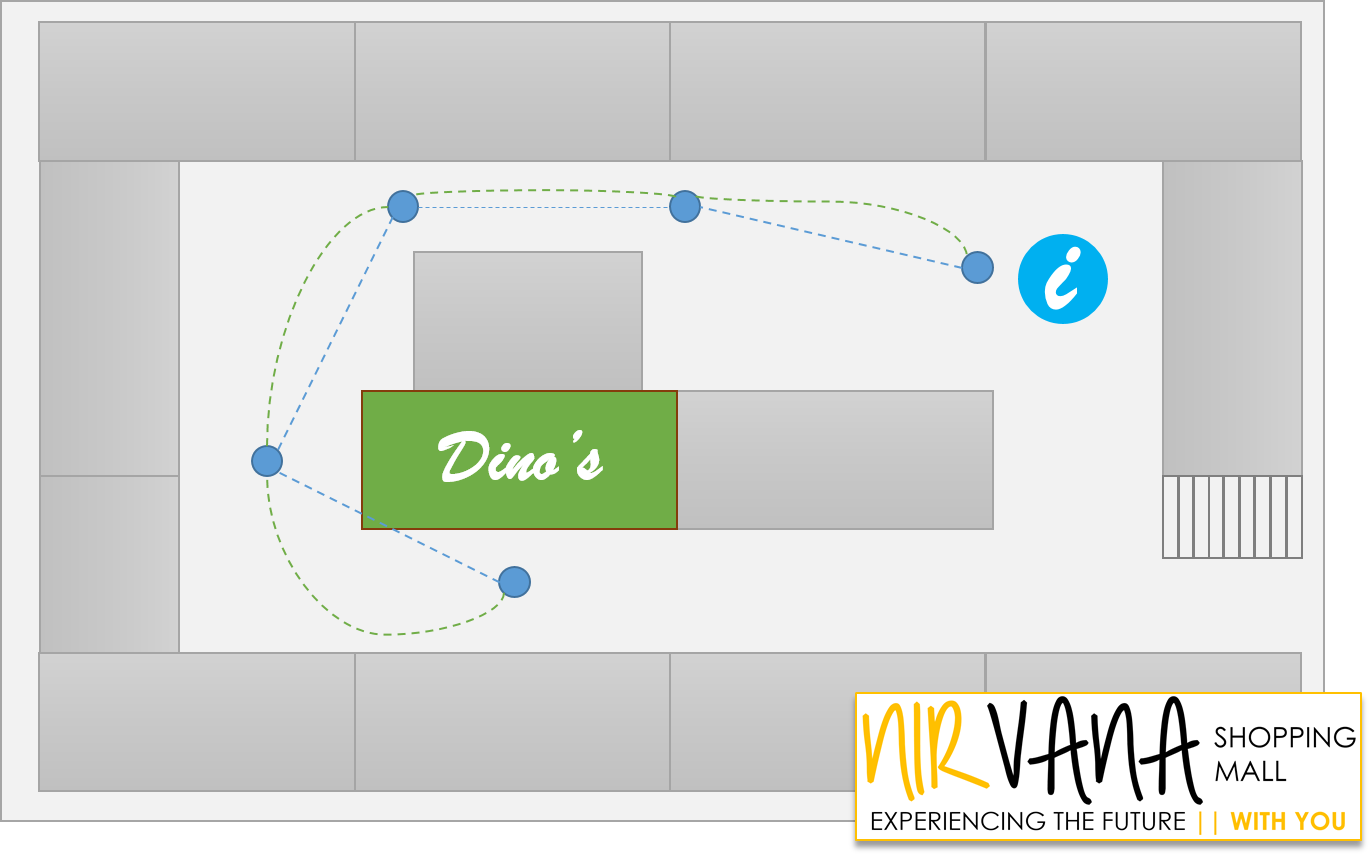
\includegraphics{mall_navigation_example2.png}
\end{figure}

    \hypertarget{formalizing-the-problem}{%
\subsection{8.2.1 Formalizing the
problem}\label{formalizing-the-problem}}

The \textbf{reactive navigation} (or \textbf{local navigation}) has the
objective of moving towards a close destination while avoiding
obstacles. For that, it is available sensor data within a specific
\emph{look-ahed} as well as the goal point (\textbf{inputs}), being the
reactive navigation method in charge of producing motor commands
(\textbf{outputs}) to safely reach such goal.

In this way, reactive navigation methods \textbf{does not require
neither any kind of map of the environment nor memory of previous
observations}. In practice, the last requirement usually arises since in
some situations it could be useful to also consider the last sensor
observations (e.g.~while crossing a door).

Finally, reactive navigation techniques \textbf{must run very fast}
(i.e.~real time or close to it) in order to safely reach the goal point.
If not, dynamic obstacles or deprecated motion commands could lead the
robot to crash!

In summary:

\begin{verbatim}
reactive_navigation(current_location,target_location,sensor_readings)
    # Method computations ... so fast!
    return (v_l,v_r) # Motor actuation
\end{verbatim}

    \hypertarget{potential-fields}{%
\subsection{8.2.2 Potential Fields}\label{potential-fields}}

\textbf{Potential Fields} is a popular and simple technique for carrying
out reactive navigation. It consist of defining a \textbf{potential
(energy) function} over the free space in the robot workspace, which has
a \textbf{global minimum} at the goal and a maximum at obstacles. Then,
in each iteration of the algorithm, the robot moves to a lower energy
configuration, similar to a a ball rolling down a hill. To carry out
such navigation the robot applies a force proportional to the
\textbf{negated gradient of the potential field} (recall that the
gradient always go in the direction in which the signal increases, and
the robot pursues a lower energy, so it has to use the negated
gradient).

The \textbf{potential (energy) function} defines a \textbf{potential
field} over the workspace. For each robot position \(q\) in such
workspace, the energy function is computed as:

\[U(q)=U_{att}(q)+U_{rep}(q)\]

where:

\begin{itemize}
\item
  \(U_{att}(q)\) is the \textbf{atractive potential field}, which is
  retrieved by:

  \[U_{att}(q)=\frac{1}{2}K_{att}\rho^2_{goal}(q)\]

  being \(\rho_{goal}\) the distance from the robot to the goal:
  \(\rho^2_{goal}=||q-q_{goal}||^2\) and \(K_{att}\) a given gain, so
  this potential is higher for far distances,
\item
  and \(U_{rep}(q)\) is the \textbf{repulsive potential field}, computed
  as:
\end{itemize}

\[U_{rep}(q)=  \begin{cases} 
   \frac{1}{2} K_{rep}(\frac{1}{\rho(q)}-\frac{1}{\rho_o})^2 & \text{if } \rho(q) < \rho_o \\
   0       & \text{if } \rho(q) \geq \rho_o
  \end{cases}\]

being \(\rho_o\) a given distance threshold, so obstacles far away from
the robot does not influence the potential field, and \(\rho(q)\) the
distance from the robot to the object.

Having defined such potential field, it can be computed a \textbf{force
field} at the robot position \(F(q)\) (a two-element vector) as the
gradient of the previous one:

\[
F(q) = -\nabla U(q) = -\nabla U_{att}(q) - \nabla U_{rep}(q) = \begin{bmatrix} \partial U / \partial x \\ \partial U / \partial y \end{bmatrix}
\]

Where: - \(-\nabla U_{att}(q)\) is also called the \textbf{attractive
force} and - \(-\nabla U_{rep}(q)\) the \textbf{repulsive force}, so -
\(F(q)=F_{att}(q)+F_{rep}(q)\).

Finally, the \textbf{robot speed (v\_x,v\_y)} is set proportional to the
force \(F(q)\) as generated by the field.

The picture below illustrates all the elements in the computation of
\(F(q)\) (\(F_{total}\) in the image, \(r\) represents \(\rho\)):

\begin{figure}
\centering
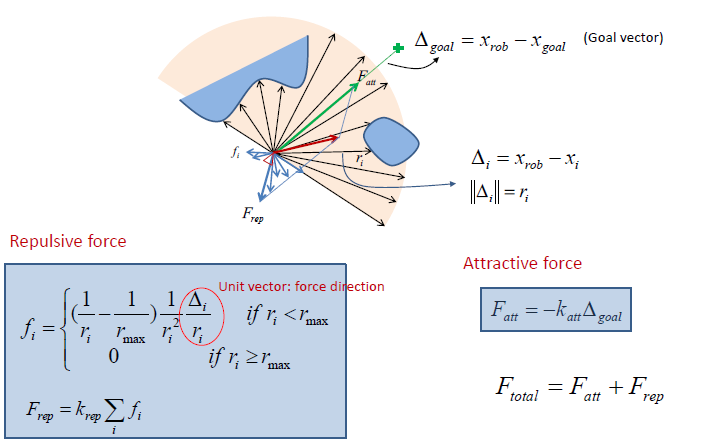
\includegraphics{potential_fields.png}
\end{figure}

    \hypertarget{developing-the-potential-fields-method-for-reactive-navigation}{%
\subsection{8.2.3 Developing the Potential Fields method for Reactive
navigation}\label{developing-the-potential-fields-method-for-reactive-navigation}}

It's time to develop our own Potential Fields method! For that, you
first need to obtain the sum of the forces that apply at a certain robot
position, computing for that the attractive and repulsive forces (recall
that \(F(q)=F_{att}(q)+F_{rep}(q)\). Then, the total force can be
retrieved, and it can be used to apply velocities to the robot wheels!

    \begin{tcolorbox}[breakable, size=fbox, boxrule=1pt, pad at break*=1mm,colback=cellbackground, colframe=cellborder]
\prompt{In}{incolor}{1}{\boxspacing}
\begin{Verbatim}[commandchars=\\\{\}]
\PY{c+c1}{\PYZsh{} IMPORTS}
\PY{k+kn}{import} \PY{n+nn}{numpy} \PY{k}{as} \PY{n+nn}{np}
\PY{k+kn}{from} \PY{n+nn}{numpy} \PY{k+kn}{import} \PY{n}{random}
\PY{k+kn}{from} \PY{n+nn}{scipy} \PY{k+kn}{import} \PY{n}{linalg}
\PY{k+kn}{import} \PY{n+nn}{matplotlib}
\PY{n}{matplotlib}\PY{o}{.}\PY{n}{use}\PY{p}{(}\PY{l+s+s1}{\PYZsq{}}\PY{l+s+s1}{TkAgg}\PY{l+s+s1}{\PYZsq{}}\PY{p}{)}
\PY{k+kn}{from} \PY{n+nn}{matplotlib} \PY{k+kn}{import} \PY{n}{pyplot} \PY{k}{as} \PY{n}{plt}

\PY{k+kn}{import} \PY{n+nn}{sys}
\PY{n}{sys}\PY{o}{.}\PY{n}{path}\PY{o}{.}\PY{n}{append}\PY{p}{(}\PY{l+s+s2}{\PYZdq{}}\PY{l+s+s2}{..}\PY{l+s+s2}{\PYZdq{}}\PY{p}{)}
\PY{k+kn}{from} \PY{n+nn}{utils}\PY{n+nn}{.}\PY{n+nn}{DrawRobot} \PY{k+kn}{import} \PY{n}{DrawRobot}
\end{Verbatim}
\end{tcolorbox}

    \hypertarget{assignment-1-computing-the-repulsive-force}{%
\subsubsection{\texorpdfstring{\textbf{{ASSIGNMENT 1: Computing the
repulsive
force}}}{ASSIGNMENT 1: Computing the repulsive force}}\label{assignment-1-computing-the-repulsive-force}}

Let's start with the repulsive force (\texttt{FRep}) computation, which
is the sum of the repulsive forces yielded by each obstacle close to the
object. Recall that forces are 2-elements column vectors.

The \texttt{repulsive\_force()} function below partially implements this
computation. Notice that this function also plots a marker over the
obstacles that have influence on this force, and store the handler of
that plot in \texttt{hInfluentialObstacles}.

Recall that:

\[
f_i=  \begin{cases} 
   (\frac{1}{\rho(q)}-\frac{1}{\rho_o}) \frac{1}{\rho(q)^2} \frac{q-q_{obj}}{\rho(q)} & \text{if } \rho(q) < \rho_o \\
   0       & \text{if } \rho(q) \geq \rho_o
  \end{cases}
  \\
F_{rep} = K_{rep} \sum_i f_i  
\]

In the code below, \(q-q_{obj}\) is stored in \texttt{q\_to\_object},
and \(\rho(q)\) in \texttt{r}. Notice that for each \(f_i\), the
distance from the robot to the object \(\rho(q)\) is a number, while
\(q-q_{obj}\) is a vector.

    \begin{tcolorbox}[breakable, size=fbox, boxrule=1pt, pad at break*=1mm,colback=cellbackground, colframe=cellborder]
\prompt{In}{incolor}{2}{\boxspacing}
\begin{Verbatim}[commandchars=\\\{\}]
\PY{k}{def} \PY{n+nf}{repulsive\PYZus{}force}\PY{p}{(}\PY{n}{xRobot}\PY{p}{,} \PY{n}{Map}\PY{p}{,} \PY{n}{RadiusOfInfluence}\PY{p}{,} \PY{n}{KObstacles}\PY{p}{)}\PY{p}{:}
    \PY{l+s+sd}{\PYZdq{}\PYZdq{}\PYZdq{} Computes the respulsive force at a given robot position}
\PY{l+s+sd}{    }
\PY{l+s+sd}{        Args:}
\PY{l+s+sd}{            xRobot: Column vector containing the robot position ([x,y]\PYZsq{})}
\PY{l+s+sd}{            Map: Matrix containing the obstacles coordinates (size 2xN\PYZus{}obstacles)}
\PY{l+s+sd}{            RadiusOfInfluence: distance threshold for considering that an obstacle has influence}
\PY{l+s+sd}{            KObstacles: gain related to the repulsive force}
\PY{l+s+sd}{        }
\PY{l+s+sd}{        Returns: Nothing. But it modifies the state in robot}
\PY{l+s+sd}{            Frep: repulsive force ([rf\PYZus{}x, rf\PYZus{}y]\PYZsq{}) (Column vector!)}
\PY{l+s+sd}{            hInfluentialObstacles: handler of the plot marking the obstacles that have influence}
\PY{l+s+sd}{    \PYZdq{}\PYZdq{}\PYZdq{}}        
    \PY{n}{q\PYZus{}to\PYZus{}object} \PY{o}{=} \PY{n}{xRobot} \PY{o}{\PYZhy{}} \PY{n}{Map}
    \PY{n}{r} \PY{o}{=} \PY{n}{np}\PY{o}{.}\PY{n}{sqrt}\PY{p}{(}\PY{n}{np}\PY{o}{.}\PY{n}{sum}\PY{p}{(}\PY{n}{q\PYZus{}to\PYZus{}object}\PY{o}{*}\PY{o}{*}\PY{l+m+mi}{2}\PY{p}{,} \PY{n}{axis}\PY{o}{=}\PY{l+m+mi}{0}\PY{p}{)}\PY{p}{)}
    \PY{n}{iInfluential} \PY{o}{=} \PY{n}{np}\PY{o}{.}\PY{n}{where}\PY{p}{(}\PY{n}{r} \PY{o}{\PYZlt{}} \PY{n}{RadiusOfInfluence}\PY{p}{)}\PY{p}{[}\PY{l+m+mi}{0}\PY{p}{]}
    
    \PY{k}{if} \PY{n}{iInfluential}\PY{o}{.}\PY{n}{shape}\PY{p}{[}\PY{l+m+mi}{0}\PY{p}{]} \PY{o}{\PYZgt{}} \PY{l+m+mi}{0}\PY{p}{:}
        \PY{n}{q\PYZus{}to\PYZus{}object} \PY{o}{=} \PY{n}{q\PYZus{}to\PYZus{}object}\PY{p}{[}\PY{p}{:}\PY{p}{,} \PY{n}{iInfluential}\PY{p}{]}
        \PY{n}{r} \PY{o}{=} \PY{n}{r}\PY{p}{[}\PY{n}{iInfluential}\PY{p}{]}
                
        \PY{n}{firstPart} \PY{o}{=} \PY{p}{(}\PY{l+m+mi}{1}\PY{o}{/}\PY{n}{r}\PY{p}{)}\PY{o}{\PYZhy{}}\PY{p}{(}\PY{l+m+mi}{1}\PY{o}{/}\PY{n}{RadiusOfInfluence}\PY{p}{)}
        \PY{n}{secndPart} \PY{o}{=}  \PY{l+m+mi}{1}\PY{o}{/}\PY{p}{(}\PY{n}{r}\PY{o}{*}\PY{o}{*}\PY{l+m+mi}{2}\PY{p}{)}
        \PY{n}{thirdPart} \PY{o}{=} \PY{p}{(}\PY{n}{q\PYZus{}to\PYZus{}object}\PY{o}{/}\PY{n}{r}\PY{p}{)}
        
        \PY{n}{f} \PY{o}{=} \PY{n}{firstPart}\PY{o}{*}\PY{n}{secndPart}\PY{o}{*}\PY{n}{thirdPart}
        
        \PY{n}{FRep} \PY{o}{=} \PY{n}{KObstacles} \PY{o}{*} \PY{n}{np}\PY{o}{.}\PY{n}{vstack}\PY{p}{(}\PY{n}{f}\PY{o}{.}\PY{n}{sum}\PY{p}{(}\PY{n}{axis}\PY{o}{=}\PY{l+m+mi}{1}\PY{p}{)}\PY{p}{)}
        
        \PY{n}{hInfluentialObstacles} \PY{o}{=} \PY{n}{plt}\PY{o}{.}\PY{n}{plot}\PY{p}{(}\PY{n}{Map}\PY{p}{[}\PY{l+m+mi}{0}\PY{p}{,}\PY{n}{iInfluential}\PY{p}{]}\PY{p}{,}\PY{n}{Map}\PY{p}{[}\PY{l+m+mi}{1}\PY{p}{,}\PY{n}{iInfluential}\PY{p}{]}\PY{p}{,}\PY{l+s+s1}{\PYZsq{}}\PY{l+s+s1}{kx}\PY{l+s+s1}{\PYZsq{}}\PY{p}{)}
    \PY{k}{else}\PY{p}{:}
        \PY{c+c1}{\PYZsh{} Nothing close}
        \PY{n}{FRep} \PY{o}{=} \PY{n}{np}\PY{o}{.}\PY{n}{vstack}\PY{p}{(}\PY{p}{[}\PY{l+m+mi}{0}\PY{p}{,}\PY{l+m+mi}{0}\PY{p}{]}\PY{p}{)}
        \PY{n}{hInfluentialObstacles} \PY{o}{=} \PY{k+kc}{None} \PY{c+c1}{\PYZsh{} Don\PYZsq{}t touch this! It is ok :)}
    
    \PY{k}{return} \PY{n}{FRep}\PY{p}{,} \PY{n}{hInfluentialObstacles}
\end{Verbatim}
\end{tcolorbox}

    \begin{tcolorbox}[breakable, size=fbox, boxrule=1pt, pad at break*=1mm,colback=cellbackground, colframe=cellborder]
\prompt{In}{incolor}{3}{\boxspacing}
\begin{Verbatim}[commandchars=\\\{\}]
\PY{c+c1}{\PYZsh{} TRY IT!}
\PY{n}{xRobot} \PY{o}{=} \PY{n}{np}\PY{o}{.}\PY{n}{vstack}\PY{p}{(}\PY{p}{[}\PY{p}{[}\PY{l+m+mi}{1}\PY{p}{]}\PY{p}{,}\PY{p}{[}\PY{l+m+mi}{2}\PY{p}{]}\PY{p}{]}\PY{p}{)}
\PY{n}{Map} \PY{o}{=} \PY{n}{np}\PY{o}{.}\PY{n}{vstack}\PY{p}{(}\PY{p}{[}\PY{p}{[}\PY{l+m+mf}{1.1}\PY{p}{,} \PY{l+m+mf}{2.4}\PY{p}{,} \PY{l+m+mf}{3.5}\PY{p}{]}\PY{p}{,}\PY{p}{[}\PY{l+m+mf}{2.2}\PY{p}{,} \PY{l+m+mf}{1.4}\PY{p}{,} \PY{l+m+mf}{4.5}\PY{p}{]}\PY{p}{]}\PY{p}{)}
\PY{n}{RadiusOfInfluence} \PY{o}{=} \PY{l+m+mi}{2}
\PY{n}{KObstacles} \PY{o}{=} \PY{l+m+mi}{200}

\PY{n}{FRep}\PY{p}{,} \PY{n}{handler} \PY{o}{=} \PY{n}{repulsive\PYZus{}force}\PY{p}{(}\PY{n}{xRobot}\PY{p}{,} \PY{n}{Map}\PY{p}{,} \PY{n}{RadiusOfInfluence}\PY{p}{,} \PY{n}{KObstacles}\PY{p}{)}

\PY{n+nb}{print} \PY{p}{(}\PY{l+s+s1}{\PYZsq{}}\PY{l+s+s1}{Repulsive force:}\PY{l+s+se}{\PYZbs{}n}\PY{l+s+s1}{ }\PY{l+s+s1}{\PYZsq{}} \PY{o}{+} \PY{n+nb}{str}\PY{p}{(}\PY{n}{FRep}\PY{p}{)}\PY{p}{)}
\end{Verbatim}
\end{tcolorbox}

    \begin{Verbatim}[commandchars=\\\{\}]
Repulsive force:
 [[ -7117.97589183]
 [-14205.83001107]]
    \end{Verbatim}

    {Expected output:}

\begin{verbatim}
Repulsive force:
 [[ -7117.97589183]
 [-14205.83001107]]
\end{verbatim}

    \hypertarget{assignment-2-retrieving-the-repulsive-force}{%
\subsubsection{\texorpdfstring{\textbf{{ASSIGNMENT 2: Retrieving the
repulsive
force}}}{ASSIGNMENT 2: Retrieving the repulsive force}}\label{assignment-2-retrieving-the-repulsive-force}}

Next, \textbf{you need to compute} the Attractive Force \texttt{FAtt}.
Do it in the \texttt{attractive\_force()} function below, taking into
account that:

\[F_{att}=-K_{att}\rho_{goal}(q)\]

Normalize the resultant Force by \(||\Delta_{goal}||\) so its doesn't
become too dominant. You can take a look at
\href{https://docs.scipy.org/doc/numpy/reference/generated/numpy.linalg.norm.html}{linalg.norm()}
for that.

    \begin{tcolorbox}[breakable, size=fbox, boxrule=1pt, pad at break*=1mm,colback=cellbackground, colframe=cellborder]
\prompt{In}{incolor}{4}{\boxspacing}
\begin{Verbatim}[commandchars=\\\{\}]
\PY{k}{def} \PY{n+nf}{attractive\PYZus{}force}\PY{p}{(}\PY{n}{KGoal}\PY{p}{,} \PY{n}{GoalError}\PY{p}{)}\PY{p}{:}
    \PY{l+s+sd}{\PYZdq{}\PYZdq{}\PYZdq{} Computes the attractive force at a given robot position}
\PY{l+s+sd}{    }
\PY{l+s+sd}{        Args:}
\PY{l+s+sd}{            KGoal: gain related to the attractive force}
\PY{l+s+sd}{            GoalError: distance from the robot to the goal ([d\PYZus{}x d\PYZus{}y]\PYZsq{})}
\PY{l+s+sd}{        }
\PY{l+s+sd}{        Returns: Nothing. But it modifies the state in robot}
\PY{l+s+sd}{            FAtt: attractive force ([af\PYZus{}x, af\PYZus{}y]\PYZsq{})}
\PY{l+s+sd}{    \PYZdq{}\PYZdq{}\PYZdq{}} 
    \PY{n}{FAtt} \PY{o}{=} \PY{o}{\PYZhy{}}\PY{n}{KGoal}\PY{o}{*}\PY{n}{GoalError}
    \PY{n}{FAtt} \PY{o}{/}\PY{o}{=} \PY{n}{linalg}\PY{o}{.}\PY{n}{norm}\PY{p}{(}\PY{n}{GoalError}\PY{p}{)} \PY{c+c1}{\PYZsh{} Normalization}
    
    \PY{k}{return} \PY{n}{FAtt}
\end{Verbatim}
\end{tcolorbox}

    \begin{tcolorbox}[breakable, size=fbox, boxrule=1pt, pad at break*=1mm,colback=cellbackground, colframe=cellborder]
\prompt{In}{incolor}{5}{\boxspacing}
\begin{Verbatim}[commandchars=\\\{\}]
\PY{c+c1}{\PYZsh{} TRY IT!}
\PY{n}{KGoal} \PY{o}{=} \PY{l+m+mf}{1.5}
\PY{n}{GoalError} \PY{o}{=} \PY{n}{np}\PY{o}{.}\PY{n}{vstack}\PY{p}{(}\PY{p}{[}\PY{p}{[}\PY{l+m+mf}{2.3}\PY{p}{]}\PY{p}{,}\PY{p}{[}\PY{l+m+mf}{1.4}\PY{p}{]}\PY{p}{]}\PY{p}{)} 

\PY{n}{FAtt} \PY{o}{=} \PY{n}{attractive\PYZus{}force}\PY{p}{(}\PY{n}{KGoal}\PY{p}{,} \PY{n}{GoalError}\PY{p}{)}

\PY{n+nb}{print} \PY{p}{(}\PY{l+s+s1}{\PYZsq{}}\PY{l+s+s1}{Attractive force:}\PY{l+s+se}{\PYZbs{}n}\PY{l+s+s1}{ }\PY{l+s+s1}{\PYZsq{}} \PY{o}{+} \PY{n+nb}{str}\PY{p}{(}\PY{n}{FAtt}\PY{p}{)}\PY{p}{)}
\end{Verbatim}
\end{tcolorbox}

    \begin{Verbatim}[commandchars=\\\{\}]
Attractive force:
 [[-1.28129783]
 [-0.77992042]]
    \end{Verbatim}

    {Expected output:}

\begin{verbatim}
Attractive force:
 [[-1.28129783]
 [-0.77992042]]
\end{verbatim}

    \hypertarget{assignment-3-concluding-with-the-total-force}{%
\subsubsection{\texorpdfstring{\textbf{{ASSIGNMENT 3: Concluding with
the Total
Force}}}{ASSIGNMENT 3: Concluding with the Total Force}}\label{assignment-3-concluding-with-the-total-force}}

Finally you can compute the Total Force \texttt{FTotal}. \textbf{Do it
in the main program below}, considering that:

\[
F_{total} = F_{att} + F_{rep}
\]

    \begin{tcolorbox}[breakable, size=fbox, boxrule=1pt, pad at break*=1mm,colback=cellbackground, colframe=cellborder]
\prompt{In}{incolor}{6}{\boxspacing}
\begin{Verbatim}[commandchars=\\\{\}]
\PY{k}{def} \PY{n+nf}{main}\PY{p}{(}\PY{n}{nObstacles}\PY{o}{=}\PY{l+m+mi}{175}\PY{p}{,}
         \PY{n}{MapSize}\PY{o}{=}\PY{l+m+mi}{100}\PY{p}{,}
         \PY{n}{RadiusOfInfluence}\PY{o}{=}\PY{l+m+mi}{10}\PY{p}{,}
         \PY{n}{KGoal}\PY{o}{=}\PY{l+m+mi}{1}\PY{p}{,}
         \PY{n}{KObstacles}\PY{o}{=}\PY{l+m+mi}{250}\PY{p}{,}
         \PY{n}{nMaxSteps}\PY{o}{=}\PY{l+m+mi}{300}\PY{p}{,}
         \PY{n}{NON\PYZus{}STOP}\PY{o}{=}\PY{k+kc}{True}\PY{p}{)}\PY{p}{:}
    
    \PY{n}{Map} \PY{o}{=} \PY{n}{MapSize}\PY{o}{*}\PY{n}{random}\PY{o}{.}\PY{n}{rand}\PY{p}{(}\PY{l+m+mi}{2}\PY{p}{,} \PY{n}{nObstacles}\PY{p}{)}
    
    \PY{n}{fig}\PY{p}{,} \PY{n}{ax} \PY{o}{=} \PY{n}{plt}\PY{o}{.}\PY{n}{subplots}\PY{p}{(}\PY{p}{)}
    \PY{n}{plt}\PY{o}{.}\PY{n}{ion}\PY{p}{(}\PY{p}{)}
    \PY{n}{ax}\PY{o}{.}\PY{n}{plot}\PY{p}{(}\PY{n}{Map}\PY{p}{[}\PY{l+m+mi}{0}\PY{p}{,}\PY{p}{:}\PY{p}{]}\PY{p}{,}\PY{n}{Map}\PY{p}{[}\PY{l+m+mi}{1}\PY{p}{,}\PY{p}{:}\PY{p}{]}\PY{p}{,}\PY{l+s+s1}{\PYZsq{}}\PY{l+s+s1}{ro}\PY{l+s+s1}{\PYZsq{}}\PY{p}{,} \PY{n}{fillstyle}\PY{o}{=}\PY{l+s+s1}{\PYZsq{}}\PY{l+s+s1}{none}\PY{l+s+s1}{\PYZsq{}}\PY{p}{)}\PY{p}{;}
    
    \PY{n}{fig}\PY{o}{.}\PY{n}{suptitle}\PY{p}{(}\PY{l+s+s1}{\PYZsq{}}\PY{l+s+s1}{Click to choose starting point:}\PY{l+s+s1}{\PYZsq{}}\PY{p}{)}
    \PY{n}{xStart} \PY{o}{=} \PY{n}{np}\PY{o}{.}\PY{n}{vstack}\PY{p}{(}\PY{n}{plt}\PY{o}{.}\PY{n}{ginput}\PY{p}{(}\PY{l+m+mi}{1}\PY{p}{)}\PY{p}{)}\PY{o}{.}\PY{n}{T}
    \PY{n+nb}{print}\PY{p}{(}\PY{l+s+s1}{\PYZsq{}}\PY{l+s+s1}{Starts at:}\PY{l+s+se}{\PYZbs{}n}\PY{l+s+si}{\PYZob{}\PYZcb{}}\PY{l+s+s1}{\PYZsq{}}\PY{o}{.}\PY{n}{format}\PY{p}{(}\PY{n}{xStart}\PY{p}{)}\PY{p}{)}
    
    
    \PY{n}{fig}\PY{o}{.}\PY{n}{suptitle}\PY{p}{(}\PY{l+s+s1}{\PYZsq{}}\PY{l+s+s1}{Click to choose end goal:}\PY{l+s+s1}{\PYZsq{}}\PY{p}{)}
    \PY{n}{xGoal} \PY{o}{=} \PY{n}{np}\PY{o}{.}\PY{n}{vstack}\PY{p}{(}\PY{n}{plt}\PY{o}{.}\PY{n}{ginput}\PY{p}{(}\PY{l+m+mi}{1}\PY{p}{)}\PY{p}{)}\PY{o}{.}\PY{n}{T}
    \PY{n+nb}{print}\PY{p}{(}\PY{l+s+s1}{\PYZsq{}}\PY{l+s+s1}{Goal at:}\PY{l+s+se}{\PYZbs{}n}\PY{l+s+si}{\PYZob{}\PYZcb{}}\PY{l+s+s1}{\PYZsq{}}\PY{o}{.}\PY{n}{format}\PY{p}{(}\PY{n}{xGoal}\PY{p}{)}\PY{p}{)}

    \PY{n}{fig}\PY{o}{.}\PY{n}{suptitle}\PY{p}{(}\PY{l+s+s1}{\PYZsq{}}\PY{l+s+s1}{\PYZsq{}}\PY{p}{)}

    \PY{n}{ax}\PY{o}{.}\PY{n}{plot}\PY{p}{(}\PY{n}{xGoal}\PY{p}{[}\PY{l+m+mi}{0}\PY{p}{,} \PY{l+m+mi}{0}\PY{p}{]}\PY{p}{,} \PY{n}{xGoal}\PY{p}{[}\PY{l+m+mi}{1}\PY{p}{,} \PY{l+m+mi}{0}\PY{p}{]}\PY{p}{,}\PY{l+s+s1}{\PYZsq{}}\PY{l+s+s1}{g*}\PY{l+s+s1}{\PYZsq{}}\PY{p}{,} \PY{n}{markersize}\PY{o}{=}\PY{l+m+mi}{10}\PY{p}{)}
    
    \PY{n}{hRob} \PY{o}{=} \PY{n}{DrawRobot}\PY{p}{(}\PY{n}{fig}\PY{p}{,} \PY{n}{ax}\PY{p}{,} \PY{n}{np}\PY{o}{.}\PY{n}{vstack}\PY{p}{(}\PY{p}{[}\PY{n}{xStart}\PY{p}{,} \PY{l+m+mi}{0}\PY{p}{]}\PY{p}{)}\PY{p}{,} \PY{n}{axis\PYZus{}percent}\PY{o}{=}\PY{l+m+mf}{0.001}\PY{p}{,} \PY{n}{color}\PY{o}{=}\PY{l+s+s1}{\PYZsq{}}\PY{l+s+s1}{blue}\PY{l+s+s1}{\PYZsq{}}\PY{p}{)}
    
    \PY{c+c1}{\PYZsh{} Initialization of useful vbles}
    \PY{n}{xRobot} \PY{o}{=} \PY{n}{xStart}
    \PY{n}{GoalError} \PY{o}{=} \PY{n}{xRobot} \PY{o}{\PYZhy{}} \PY{n}{xGoal}
    
    \PY{c+c1}{\PYZsh{} Simulation}
    \PY{n}{k} \PY{o}{=} \PY{l+m+mi}{0}

    \PY{k}{while} \PY{n}{linalg}\PY{o}{.}\PY{n}{norm}\PY{p}{(}\PY{n}{GoalError}\PY{p}{)} \PY{o}{\PYZgt{}} \PY{l+m+mi}{1} \PY{o+ow}{and} \PY{n}{k} \PY{o}{\PYZlt{}} \PY{n}{nMaxSteps}\PY{p}{:}

        \PY{n}{FRep}\PY{p}{,} \PY{n}{hInfluentialObstacles} \PY{o}{=} \PY{n}{repulsive\PYZus{}force}\PY{p}{(}\PY{n}{xRobot}\PY{p}{,} \PY{n}{Map}\PY{p}{,} \PY{n}{RadiusOfInfluence}\PY{p}{,} \PY{n}{KObstacles}\PY{p}{)}
        \PY{n}{FAtt} \PY{o}{=} \PY{n}{attractive\PYZus{}force}\PY{p}{(}\PY{n}{KGoal}\PY{p}{,} \PY{n}{GoalError}\PY{p}{)}
                
        \PY{c+c1}{\PYZsh{} Point 1.3}
        \PY{c+c1}{\PYZsh{} TODO Compute total (attractive+repulsive) potential field}
        
        \PY{n}{FTotal} \PY{o}{=} \PY{n}{FAtt} \PY{o}{+} \PY{n}{FRep}
        \PY{c+c1}{\PYZsh{}FTotal /= linalg.norm(FTotal)}
        
        \PY{n}{xRobot} \PY{o}{+}\PY{o}{=} \PY{n}{FTotal}
        \PY{n}{Theta} \PY{o}{=} \PY{n}{np}\PY{o}{.}\PY{n}{arctan2}\PY{p}{(}\PY{n}{FTotal}\PY{p}{[}\PY{l+m+mi}{1}\PY{p}{,} \PY{l+m+mi}{0}\PY{p}{]}\PY{p}{,} \PY{n}{FTotal}\PY{p}{[}\PY{l+m+mi}{0}\PY{p}{,} \PY{l+m+mi}{0}\PY{p}{]}\PY{p}{)}
        
        \PY{n}{hRob}\PY{o}{.}\PY{n}{pop}\PY{p}{(}\PY{l+m+mi}{0}\PY{p}{)}\PY{o}{.}\PY{n}{remove}\PY{p}{(}\PY{p}{)}
        \PY{n}{hRob} \PY{o}{=} \PY{n}{DrawRobot}\PY{p}{(}\PY{n}{fig}\PY{p}{,} \PY{n}{ax}\PY{p}{,} \PY{n}{np}\PY{o}{.}\PY{n}{vstack}\PY{p}{(}\PY{p}{[}\PY{n}{xRobot}\PY{p}{,} \PY{n}{Theta}\PY{p}{]}\PY{p}{)}\PY{p}{,} \PY{n}{axis\PYZus{}percent}\PY{o}{=}\PY{l+m+mf}{0.001}\PY{p}{,} \PY{n}{color}\PY{o}{=}\PY{l+s+s1}{\PYZsq{}}\PY{l+s+s1}{blue}\PY{l+s+s1}{\PYZsq{}}\PY{p}{)}
        
        \PY{k}{if} \PY{n}{NON\PYZus{}STOP}\PY{p}{:}
            \PY{n}{plt}\PY{o}{.}\PY{n}{pause}\PY{p}{(}\PY{l+m+mf}{0.1}\PY{p}{)}
        \PY{k}{else}\PY{p}{:}
            \PY{n}{plt}\PY{o}{.}\PY{n}{waitforbuttonpress}\PY{p}{(}\PY{o}{\PYZhy{}}\PY{l+m+mi}{1}\PY{p}{)}
            
        \PY{k}{if} \PY{n}{hInfluentialObstacles} \PY{o+ow}{is} \PY{o+ow}{not} \PY{k+kc}{None}\PY{p}{:}
            \PY{n}{hInfluentialObstacles}\PY{o}{.}\PY{n}{pop}\PY{p}{(}\PY{l+m+mi}{0}\PY{p}{)}\PY{o}{.}\PY{n}{remove}\PY{p}{(}\PY{p}{)}
        
        \PY{c+c1}{\PYZsh{} Update termination conditions}
        \PY{n}{GoalError} \PY{o}{=}  \PY{n}{xRobot} \PY{o}{\PYZhy{}} \PY{n}{xGoal}
        \PY{n}{k} \PY{o}{+}\PY{o}{=} \PY{l+m+mi}{1}
\end{Verbatim}
\end{tcolorbox}

    \hypertarget{understanding-how-the-technique-performs}{%
\subsection{8.2.4 Understanding how the technique
performs}\label{understanding-how-the-technique-performs}}

As a brilliant engineer, you have to provide some indications to the
\textbf{{managers at Nirvana}} about how the technique performs and its
limitations, which has to be provided in the next Thinking about it. The
following code cells help you to execute the implemented technique with
different parameters in order to retrieve the required information.

    \begin{tcolorbox}[breakable, size=fbox, boxrule=1pt, pad at break*=1mm,colback=cellbackground, colframe=cellborder]
\prompt{In}{incolor}{ }{\boxspacing}
\begin{Verbatim}[commandchars=\\\{\}]
\PY{c+c1}{\PYZsh{} For considering different gains}
\PY{n}{main}\PY{p}{(}\PY{n}{KGoal}\PY{o}{=}\PY{l+m+mi}{1}\PY{p}{,} \PY{n}{KObstacles}\PY{o}{=}\PY{l+m+mi}{250}\PY{p}{)}
\PY{c+c1}{\PYZsh{} main(KGoal=1, KObstacles=250, nObstacles = 50)}
\end{Verbatim}
\end{tcolorbox}

\begin{figure}
\centering
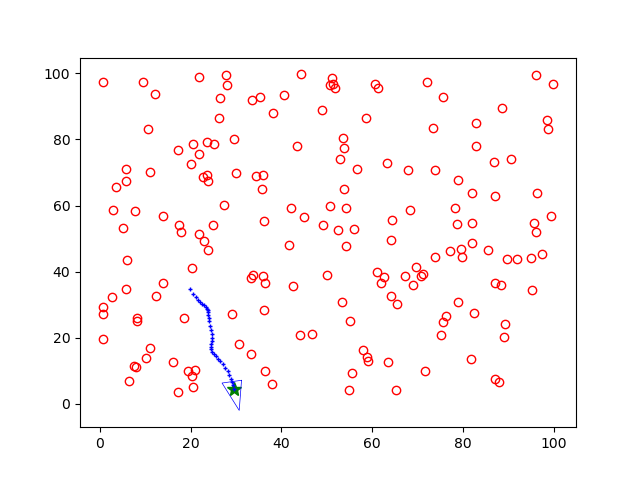
\includegraphics{Ex1_1.png}
\end{figure}

    \begin{Verbatim}[commandchars=\\\{\}]
Starts at:
[[19.83429013]
 [34.69308748]]
Goal at:
[[29.53686931]
 [ 4.43293224]]
    \end{Verbatim}

    \begin{tcolorbox}[breakable, size=fbox, boxrule=1pt, pad at break*=1mm,colback=cellbackground, colframe=cellborder]
\prompt{In}{incolor}{ }{\boxspacing}
\begin{Verbatim}[commandchars=\\\{\}]
\PY{c+c1}{\PYZsh{} For considering different number of obstacles}
\PY{n}{main}\PY{p}{(}\PY{n}{nObstacles}\PY{o}{=}\PY{l+m+mi}{175}\PY{p}{)}
\end{Verbatim}
\end{tcolorbox}

\begin{figure}
\centering
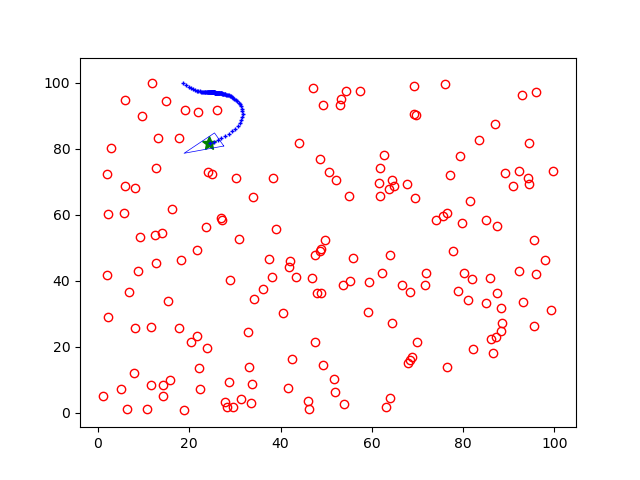
\includegraphics{Ex1_2.png}
\end{figure}


    \begin{Verbatim}[commandchars=\\\{\}]
Starts at:
[[ 18.63957661]
 [100.01438567]]
Goal at:
[[24.33503591]
 [81.69901372]]
    \end{Verbatim}

    \hypertarget{thinking-about-it-1}{%
\subsubsection{Thinking about it (1)}\label{thinking-about-it-1}}

\textbf{Address the following points} to gain insight into how the
developed Potential Fields technique performs. You can include some
figures if needed.

\begin{itemize}
\item
  Discuss the meaning of each element appearing in the plot during the
  simulation of the \emph{Potential Fields reactive navigation}.
  \(\\[10pt]\)

\begin{figure}
\centering
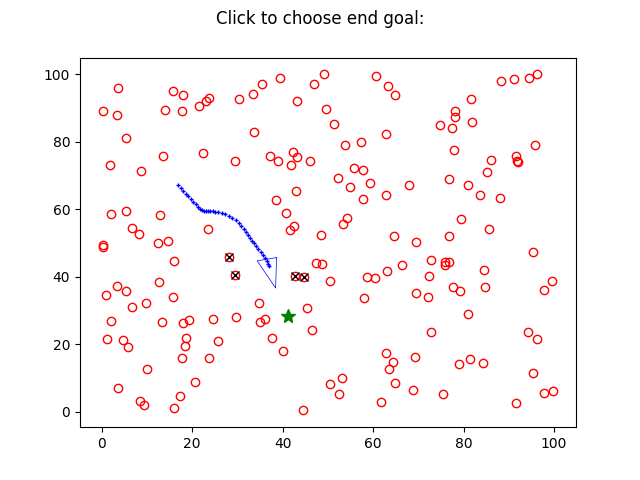
\includegraphics{fig8-1-2.png}
\end{figure}

  Red dots are the obstacles in the map. The blue triangle is our robot.
  Red dot with a black cross are the obstacles that their repulsive
  force affects to the robot. The green star is the goal position and
  the blue trace are the movements that the robot did.
\item
  Run the program setting different start and goal positions. Now change
  the values of the goal and obstacle gains (\texttt{KGoal} and
  \texttt{KObstacles}). How does this affect the paths followed by the
  robot?

  Examples with different values for such constants:

\begin{figure}
\centering
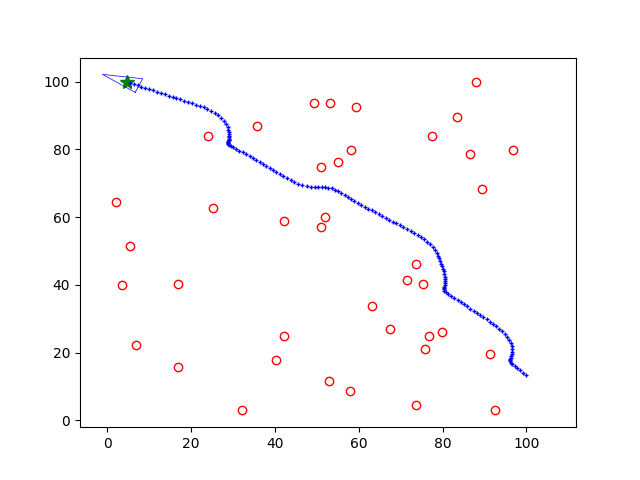
\includegraphics{fig8-1-3.png}
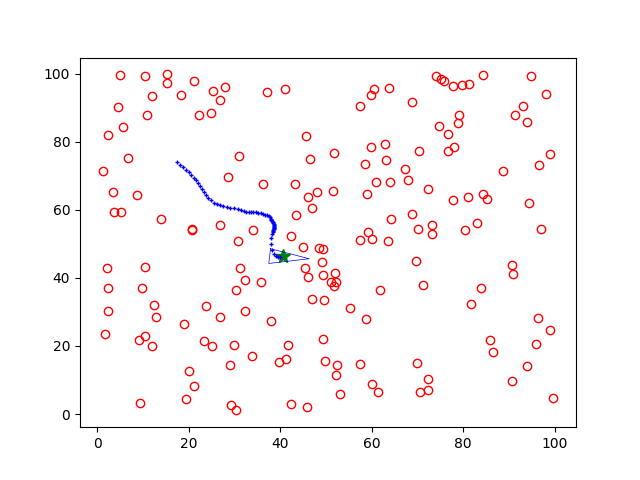
\includegraphics{fig8-1-4.png}
\end{figure}

  If we increase goal gain value, the robot will be more attracted to
  the goal, and will go faster to the goal, sometimes skipping
  obstacles. If we increase obstacles gains values, the robot will found
  more difficult to reach the goal.
\item
  Play with different numbers of obstacles and discuss the obtained
  results.

  With less obstacles, the robot will probably reach more quickly the
  goal. However, if we increase the number of obstacles, the robot will
  found more difficult to reach the goal and is more probably to get
  stucked.
\item
  Illustrate a navigation where the robot doesn't reach the goal
  position in the specified number of steps. Why did that happen? Could
  the robot have reached the goal with more iterations of the algorithm?
  Hint: take a look at the \texttt{FTotal} variable.

  No, the robot got stucked. This happens because the sum of the FAttr
  and FRep 0 or very close to 0. This makes the robot to not to move.
\end{itemize}


    % Add a bibliography block to the postdoc
    
    
    
\end{document}
